\begin{figure}[ht]
    \centering
    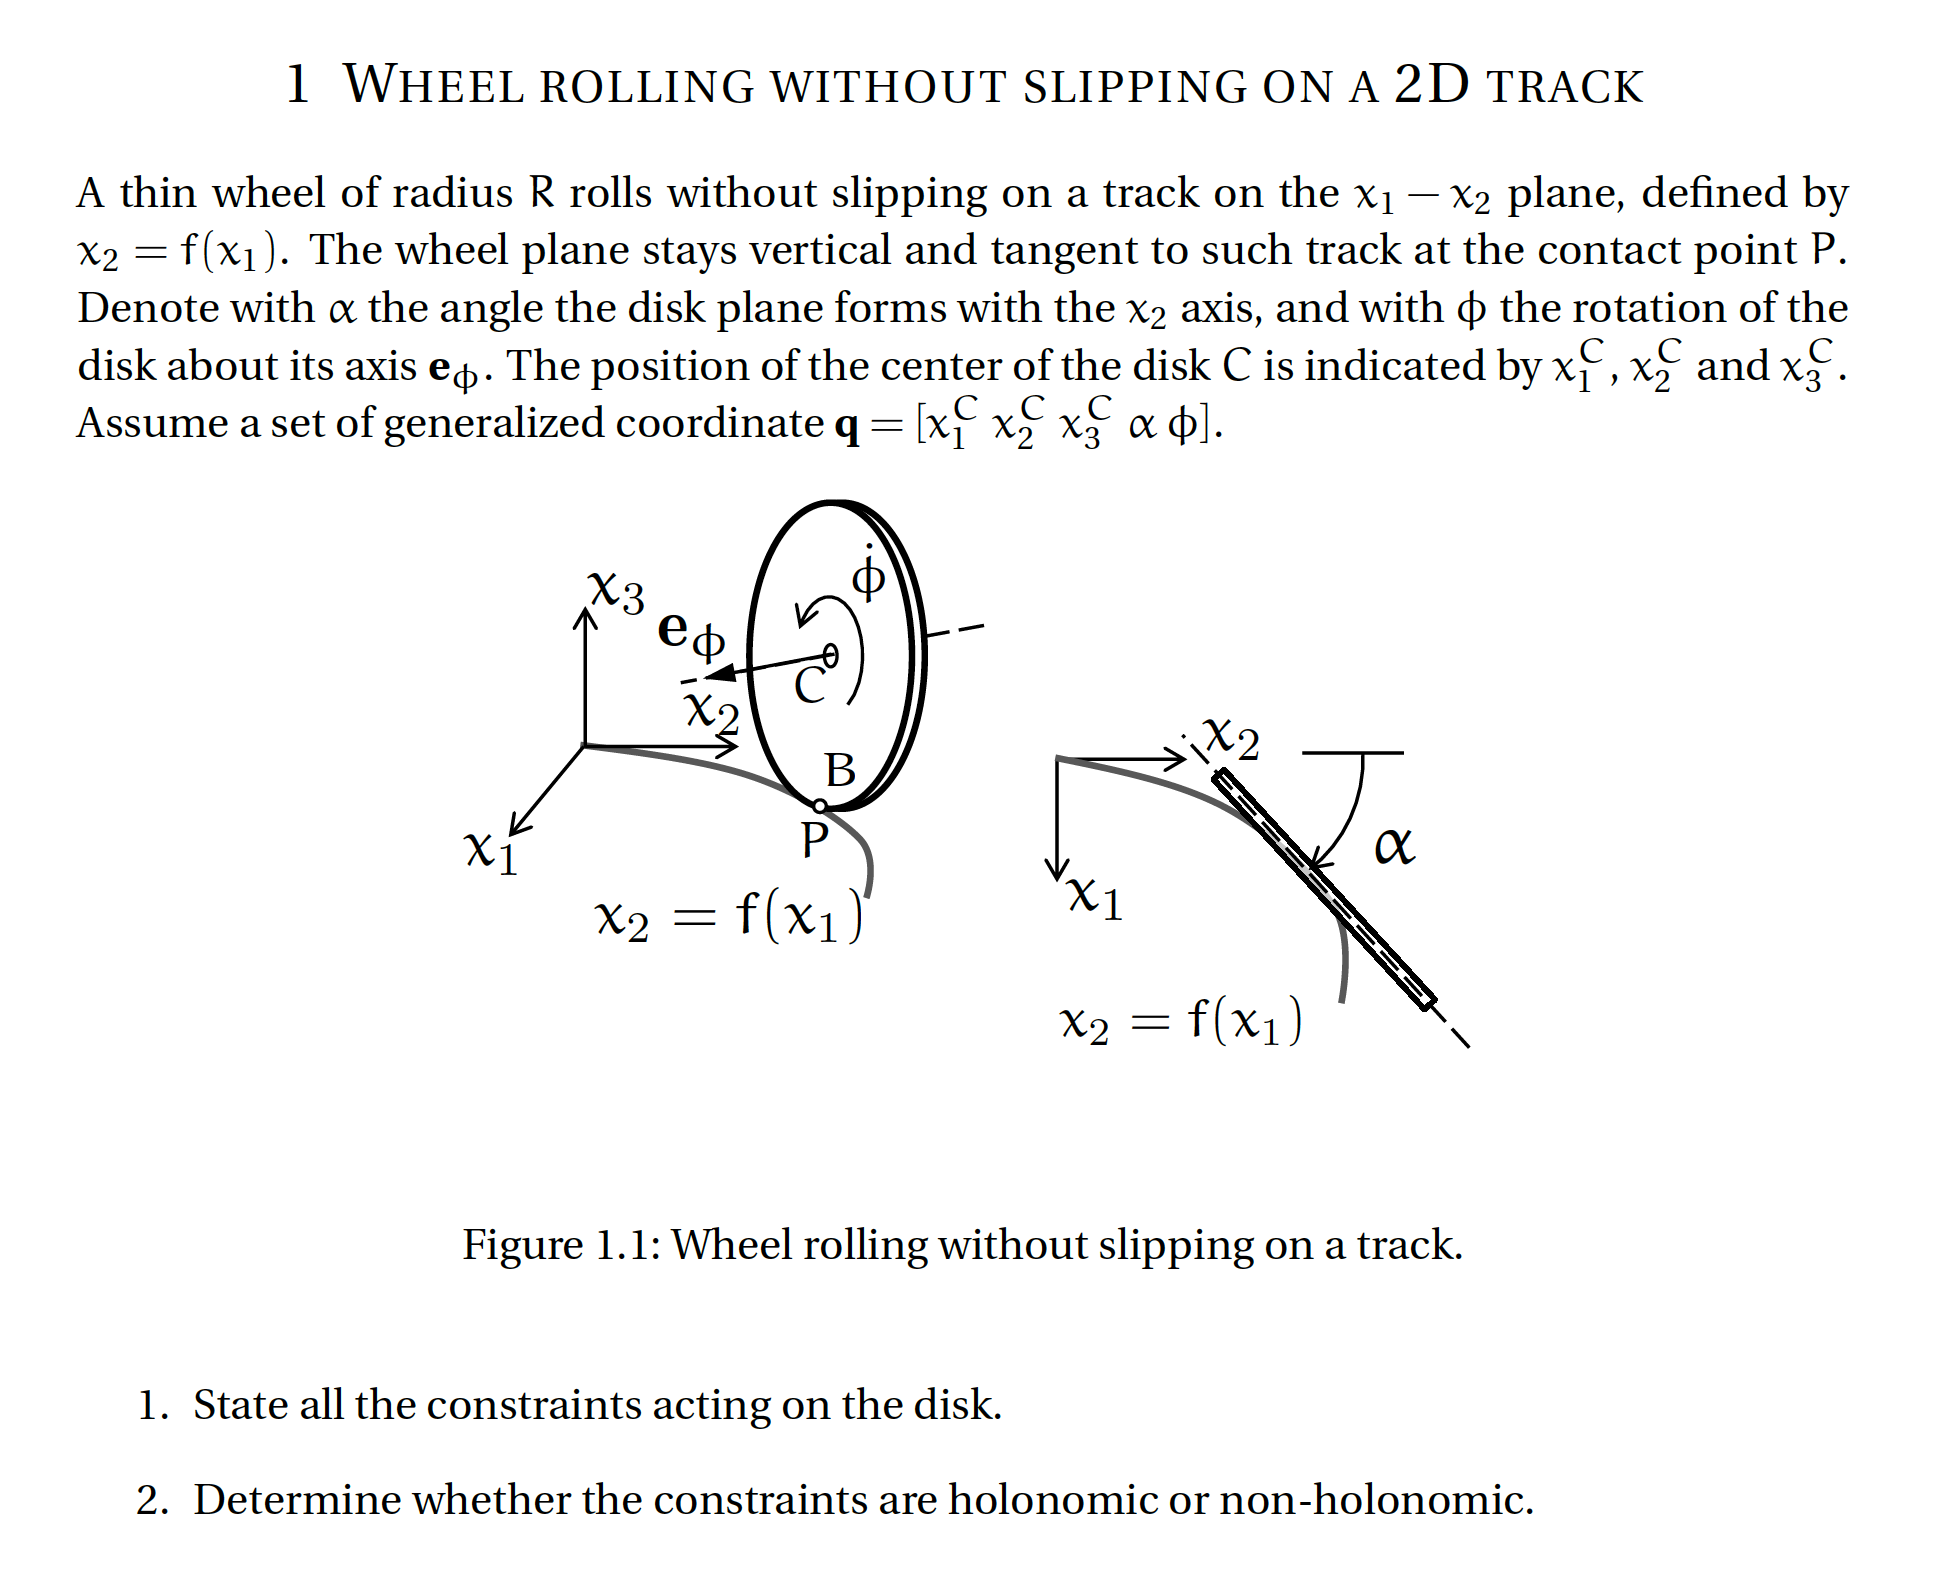
\includegraphics[scale=0.4]{images/1.1.png}
    \caption{Task 1.1}
    %label always in the end
    \label{fig:task1.1}
\end{figure}
\clearpage

\subsection{}
The list of constraints looks as follows:

\begin{enumerate}
    \item The wheel always stays vertical (plane parallel to $x_3$)\\
        This is a holonomic constraint: $f = \theta = 0$ where $\theta$ denotes the angle between the disk and $x_3$
    \item $x_2$ follows a fixed trajectory, given $x_1$ (and vice versa):\\
        $f_2: x_2 = f(x_1) \Rightarrow x_2 - f(x_1) = 0 \Rightarrow$ holonomic.
    \item $\alpha$ is the angle between the trajectory and the $x_2$ axis:\\
        $\alpha = \frac{\pi}{2} - \frac{\partial f(x_1)}{\partial x_1}$ or written differently:\\
             $f(\alpha, x_1) = \alpha - \frac{\pi}{2} + \frac{\partial f(x_1)}{\partial x_1} = 0 \Rightarrow$ holonomic
    \item Rolling without slipping:\\
        $v_B = 0 \Rightarrow v_C + \omega \times R_{CB} = 0$ with $\omega = \dot{\alpha}\boldsymbol{e_3} + \dot\phi\boldsymbol{e_\phi}$\\
        Seems to be non-holonomic at first glance
    \item The disk does not leave the ground:\\
        $x_3^C - R = 0$ aka the $x_3$ component of the center of mass is R.\\
        This is holonomic as well
\end{enumerate}

\noindent So far we have a 3D system (6 DoF) and 4 holonomic constraints and 1 non-holonomic constraint.\vspace{1cm}

4. Check for integrability:
\Huge \color{red}To Do \color{black}\normalsize
\begin{equation}
    \begin{split}
        &v_B = 0 \Rightarrow v_C + \omega \times R_{CB} = 0\\
    \end{split}
\end{equation}
Plugging in $\dot{x}_1^C, \dot{x}_2^C, \omega = \dot{\alpha}\boldsymbol{e_3} + \dot\phi\boldsymbol{e_\phi} \text{ and } R_{CB} = [0,0,-R]^T$:
\begin{equation}
    \begin{split}
        &\dot x_1^C\boldsymbol{e_1} + \dot x_2^C\boldsymbol{e_2} -  R\dot\phi\cos\alpha\boldsymbol{e_2} - R\dot\phi\sin\alpha\boldsymbol{e_1} = 0
    \end{split}
\end{equation}

Considering the part in $\boldsymbol{e_1}$ direction:
\begin{equation}
    \begin{split}
        &\dot x_1^C - R\dot\phi\sin\alpha = 0 
    \end{split}
\end{equation}
Now if we reformulate this in the linear velocity form:
\begin{equation}
    \sum_{i=1}^n a_i(\boldsymbol{q},t)\dot q_i + b(\boldsymbol{q},t) \text{ with \textbf{q} = }[x_1^C,x_2^C, x_3^C,\alpha, \phi]
\end{equation}
We get
\begin{equation}
    \begin{split}
        &a_1 = 1, \quad a_5 = -R\sin(\alpha), b = 0\\
        &\Rightarrow \frac{\partial(Cb)}{\partial q_1} = \frac{\partial(Ca_1)}{\partial t} \Rightarrow \frac{\partial C}{\partial t} = 0 \Rightarrow C \neq C(t)\\
        &\Rightarrow \frac{\partial(Ca_1)}{\partial q_5} = \frac{\partial(Ca_5)}{\partial q_1} \Rightarrow \frac{\partial(C)}{\partial \phi} = \frac{\partial(-CR\sin(\alpha))}{\partial x_1^C}\\
        & \Rightarrow \frac{\partial(C)}{\partial \phi} = -R\sin(\alpha)\frac{\partial(C)}{\partial x_1^C}
    \end{split}
\end{equation}
Perhaps we can show directly that the constraint can be written in the solution form:
\begin{equation}
    \begin{split}
        \dot x_1^C\boldsymbol{e_1} - R\dot\phi\sin\alpha\boldsymbol{e_1} = \sum_{i=1}^n \frac{\partial f(\boldsymbol{q},t)}{x_1^C}\dot x_1^C + \frac{\partial f(\boldsymbol{q},t)}{\phi}\dot \phi
    \end{split}
\end{equation}
\subsection{}
See section 1.1
\subsection{}

\begin{figure}[ht]
    \centering
    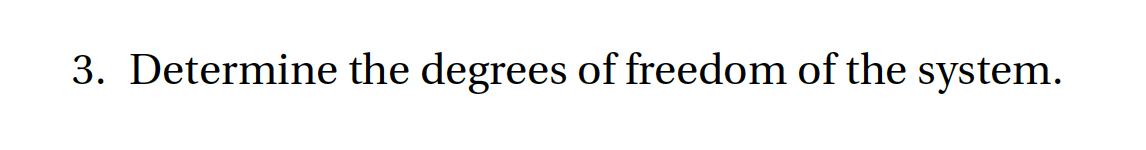
\includegraphics[scale=0.4]{images/1.1.3.png}
    \caption{Task 1.1.3}
    %label always in the end
    \label{fig:task1.1.3}
\end{figure}

\noindent As we have a 3D body with 6 generalized coordinates (here 5 are given, already considering constraint 1) and 5 holonomic constraints. We get a total of $6 - 5 = 1$ degree of freedom. That could for instance be the rotation of the wheel around $\boldsymbol{e_\phi}$ while all the other generalized coordinates follow accordingly.

